\newpage
\renewcommand{\TheTitle}{Efficient Preconditioning for Space-Parallel One Cell Inversions in Slab Geometry using a Second Moment Method}
\renewcommand{\TheAuthors}{Joanna Piper Morgan,
  Todd S. Palmer,
  Ilham Variansyah, and
  Kyle E. Niemeyer}

\renewcommand{\TheAddress}{%
    In preparation for submission
}

\PaperHeader{\TheTitle}{\TheAuthors}{\TheAddress}

\chapter{\TheTitle}
\label{chap:smom_paper}

\epigraphhead[10]{\singlespacing
    \epigraph{
        We are responsible for the world in which we find ourselves, if only because we are the only sentient force which can change it.
    }
    {James Baldwin}
}
% Communications of the ACM, Sept. 1985

\newcommand{\dxt}{\frac{\Delta x_j}{2}}
\newcommand{\mum}{\mu_m}

\newcommand{\Lc}{\bm{L}_c}
\newcommand{\Lb}{\bm{L}_b}

\newcommand{\scat}{\sigma_s}
\newcommand{\tot}{\sigma}
\newcommand{\abs}{\sigma_a}

\newcommand{\la}{^{(l)}}

\newcommand{\af}{\psi}
\newcommand{\sfl}{\phi}
\newcommand{\smom}{\Gamma}
\newcommand{\fmom}{J_\pm}
\newcommand{\fmomp}{J_+}
\newcommand{\fmomn}{J_-}

\newcommand{\ddx}{\frac{\partial}{\partial x}}
\newcommand{\ddxn}{\frac{d}{d x}}

\newcommand{\sn}{S$_N$}
\newcommand{\pn}{P$_N$}

\newcommand{\half}{\frac{1}{2}}


\section*{Abstract}
Solving the S$_N$ radiation transport equation on modern many-core compute architectures (i.e., GPUs) is challenging.
The most common implemented solution method, source iteration, requires computationally expensive sweeping operations that cannot be parallelized in 1D.
While in 2D and 3D sweeps can use full parallel sweeping algorithms, these schemes may not perform well on a GPU.
One cell inversion (OCI) is another class of solvers for the radiation transport equation.
OCI iterations are parallel over spatial cells, which has been previously shown to out-perform similarly implemented versions of unpreconditioned source iterations on GPUs for some problems.
While OCI rapidly converges for optically thick problems, spectral radius tends to one in both the optically thin and diffusive limits.
Finding a preconditioner for OCI to support converging in these regimes that can also be efficiently computed on many-core architectures motivates this work.
%We have previously shown that for time dependent problems OCI's spectral radius has an added dependence on mean free time and tends to zero as mean free time decreases.
We derive a second moment cellular decomposition method in conjunction with OCI iteration in an effort to produce a fully space-parallel, rapidly convergent, transport iteration.
The second moment preconditioner derived in this work does not converge to the same solution as unpreconditioned transport solutions, suggesting inconsistencies in the numerical scheme.
Numerical experiments show the second moment preconditioner rapidly converges in the thick diffusive limit but does not aid convergence in the optically thin limit.

\section{Introduction}

The radiation transport equation is a linear integro-partial differential equation that describes the movement of neutral particles (photons, neutrons, phonons, and neutrinos) in seven independent variables (space, velocity, and time).
Applications of the transport equation include nuclear reactor physics \cite{duderstadt_hamilton}, heat transfer \cite{radheattrans2003}, health physics \cite{martelli_2010_light}, and astrophysics \cite{chandrasekhar1960radiative}.
The transport equation is often solved with either a Monte Carlo or a deterministic method, or some combination between the two \cite{lewis_computational_1984}.
Monte Carlo methods can be prohibitively slow to converge for high-fidelity transient problems, requiring huge numbers of simulated particles to converge to a statistically significant solution \cite{lux_1998}.
Deterministic methods are usually able to reach solution faster for the same problem modeled in similar fidelity, but can be much more sensitive to implemented physics and restrict what type of problems a particular method can solve \cite{lewis_computational_1984}. 
The high dimensionality of transport equations means that computationally and memory efficient iterative methods are often used as a primary solution method \cite{adams_fast_2002}.
As GPUs continue to become the dominant computational workhorse in science and engineering they are allowing for fully time-dependent solutions to the transport equation.
Finding efficient and rapidly convergent numerical methods for modern high performance computers is paramount.

Deterministic methods for solving the radiation transport equation are commonly divided into one of two categories: the method of spherical harmonics (\pn) and the method of discrete ordinance (\sn).
Both turn the Boltzmann-type integro-differential transport equation into an infinite set of coupled partial differential equations and solves a finite number of them.
The \pn method does this by taking angular moments of the transport equation then making a closure assumption.
The \sn method, first described by Chandrasekhar for radiation transport in stellar media, treats the double integral over both angular directions with a quadrature discretization \cite{chandrasekhar1960radiative}.
In the \sn method, each differential equation in the finite set solves along a particular angular direction; in solid angle provided from a finite quadrature.
In a single dimension solutions to the \sn and \pn methods of a given order are the same.
In higher spatial dimensions they are not, and the \sn method suffers from ``ray effects" as there is no way to map a quadrature set to perfectly integrate over a circle or sphere. % needs a citation blah


\section{Transport Iterations}

Source iterations (SI) are widely used to solve the \sn neutron transport equation \cite{adams_fast_2002}.
The source iteration is a specific type of operator splitting of the linear neutron transport equation where the scattering term---which couples all \sn ordinates together---is lagged to information from a previous iteration \cite{lewis_computational_1984}.
SI is embarrassingly parallel over angle space, which can prove inefficient for large computers as there are usually fewer degrees of freedom in angle than in space.
The SI method requires a transport ``sweep" to spatially move through the problem in a specific non-parallelizable order in 1D.
While memory-efficient parallel 2D and 3D SI schemes ezetast (namely Koch--Baker--Alcouff (KBA) or full parallel sweeps (FPS) \cite{baker_computational_2017, baker_kba_2017, alcouffe_time-dependent_1998} algorithm), they are difficult to implement and may not be efficient on GPUs.
Available performance results for full parallel sweeps on GPUs show that even optimized applications under-perform relative to the theoretical hardware resources available \cite{Thomas_2024_profiling, wolfe2022roofline, kunen_kripke_2015, zerr_partisn_2019}.
Finding a rapidly convergent space-parallel iteration scheme could prove beneficial to performance on modern many-core compute architectures (i.e., GPUs).

A one cell inversion (OCI) is an alternative to a source iteration where incident angular fluxes on the surface of the cell are lagged and each cell is solved independently of every other cell \cite{rosa_cellwise_2013, adams_fast_2002}.
Depending on the order of the inversion the iterations can look like a cell-wise block Jacobi, cell-wise block Gauss--Seidel, or red--black iterations \cite{man1994parallel}.
However, OCI fails to converge in the thin limit with spectral radius ($\rho$) tending to unity as cellular optical thickness ($\delta=\Sigma\Delta x$ in mean free path) decreases ($\lim_{\delta\rightarrow0}(\rho) = 1$) \cite{tsa_slab2006rosa}.
Physically this can be understood as the requirements of communication from cell-to-cell.
Information can only pass through a single cell in a given iteration.
So a problem with more cells will require more iterations to communicate information than the same problem with fewer cells.
Mathematically this is understood as the decreasing diagonal-dominance of the iteration systems present in OCI algorithms, where Jacobi or Gauss-Seidel iteration schemes take longer to converge \cite{isaacson_numerical_1966}.
Previously this has been described as asynchronicity in space \cite{hoagland_hybrid_2021}.
OCI can diverge in the diffusive (scattering) limit.

We have previously shown that on modern GPUs when space is the dominant dimension, OCI can out-perform SI in wall clock runtime up to a point in the thin and diffusive limits \cite{morgan2023oci}.
In these circumstances OCI may require more iterations to converge a problem; however, OCI iterations can done much faster on a GPU than similarly implemented SI algorithms.
The OCI algorithm requires the solution to many relatively small linear algebra systems (in the orders of 8--100) in each cell, which is a highly compute-bound operation that can be done efficiently on GPUs using library operations \cite{morgan_2025_oci}.
We have also previously shown that adding time resolution to OCI iterations can resynchronize cells and make OCI convergent for problems in the thin and diffusive limits where in steady state OCI can be nonconvergent.
For time-dependent OCI spectral radii approach zero as mean free time decreases \cite{morgan_2025_oci}.
Time resolution is a benefit to convergence for both SI and OCI algorithms.
However, OCI has a compounding benefit: its additional dependency on the cellular optical thickness---which itself is inversely proportional to mean free time.

Figure \ref{fig:ss_spec_rads} shows spectral radii of unpreconditioned SI (left) and unpreconditioned OCI (middle) over choices of cellular optical thickness ($\delta$) and scattering ratio ($c$) computed from Fourier analysis of an infinite homogeneous medium problem in S$_8$\footnote{Gauss--Legendre quadrature is used in all work presented.}.
Unprecondtioned SI depends linearly on $c$, and for the infinite homogeneous medium problem does not depend on $\delta$.
OCI depends both on scattering ratio and cellular optical thickness---being rapidly convergent in the thick limit ($\delta>1.0$) with degrading spectral properties towards the thin and diffusive limits ($\delta<1.0$ and $c>0.95$).

\begin{figure}
    \centering
    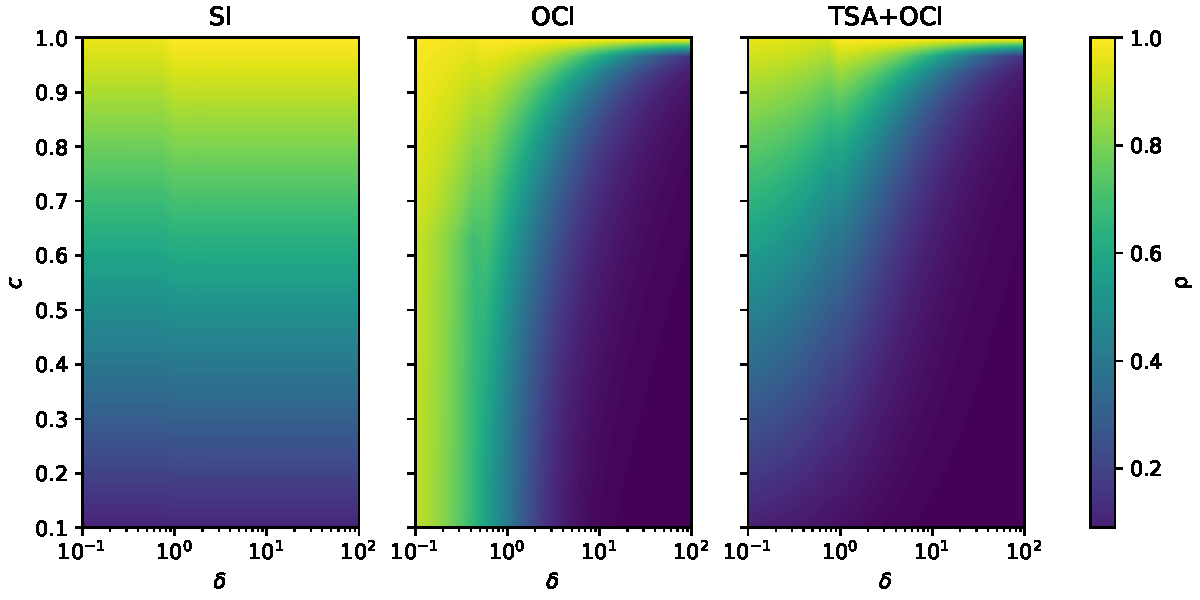
\includegraphics[width=\linewidth]{figures/smm_paper/ss_specrads.pdf}
    \caption{Spectral radii ($\rho$) of (left) unpreconditioned SI, (center) unpreconditioned OCI, and (right) OCI with transport synthetic acceleration ($\beta=1.0$), over ranges of scattering ratio $c$ and cellular optical thickness ($\delta$) in S$_8$ and 200 choices of wave mode $\in[0,2\pi]$. }
    \label{fig:ss_spec_rads}
\end{figure}

Preconditioners can be used to aid convergence of iterative schemes for the neutron transport equation \cite{adams_fast_2002}.
Often physics-informed preconditioners for transport iterations may be thought of as a high-order method solving the full discretized transport equation and a low-order method informing intra-iteration updates to then be used in the next iteration of the high-order problem.
The low-order method is usually some physics-informed problem that is computationally cheaper to solve than the transport problem and models physical behavior that is difficult for a given operator splitting to converge (e.g., the diffusive limit, $c\rightarrow1$).

Synthetic acceleration schemes are a common subset of preconditioners for the SI operator splitting.
A synthetic acceleration method only \textit{accelerates} convergence to the same solution as transport and is fully consistent with the high-order transport method.
Generally for synthetic acceleration methods the low-order simulation is \textit{driven} by the error between iterations of a transport solve.
Synthetic acceleration techniques for source iterations include:
boundary projection acceleration \cite{adams_boundary_1988}, 
transport synthetic acceleration \cite{ramone_1997_tsa},
multi-grid methods \cite{man1994parallel},
and the venerable diffusion synthetic acceleration (DSA) \cite{larsen_1983_dsaforsn}, among others.

Diffusion synthetic acceleration is a common preconditioner for the source iteration operator splitting \cite{adams_fast_2002, alcouffe_1977_dd, coale_2025_dsa}.
It implements a low-order diffusion solve driven by the error between subsequent transport iterations to inform a correction term for the scalar flux, which can in turn be used as the source in a subsequent high-order source iteration.
To make DSA consistent the specific structures of the low-order diffusion solve is governed by the spatial discretization scheme used in the high-order transport simulation.
Larsen's four-step method can be used to yield a DSA scheme that is consistent with spatial discretization, however, the system of equations produced from a Larsen four-step process can be difficult to solve, or form inconsistent schemes for finite elements in higher dimensions \cite{larsen_1982_unconDSA, larsen_1982_unconDSAte, haut_2020_dsa}. 
The Adams--Martin modified four-step process produces consistent schemes with finite element discretization methods \cite{adams_1992_dsadfe}.
Consistent DSA-SI schemes produce rapidly convergent iteration methods where $\rho<c/3$ in homogeneous regions.

Another class of physics-informed preconditioners for the radiation transport equation that do not fall into the sub-category of synthetic acceleration are the moment expansion methods including: second moment (also called Lewis \& Miller methods) \cite{olivier_2024_smoms, lewis_computational_1984, oliver_2025_secondmoment}, quasi-diffusion \cite{ani_1986_quasidiffusion, goldin_1964_quasidissuion}, and variable Eddington factor \cite{lou_2021_vef, coale_2024_rmomvef} methods.
All of these preconditioners are themselves a set of high-low (HOLO) methods \cite{chacon_2017_holosurvey}.
They still use the same general algorithm as synthetic acceleration where information from the high-order transport solve somehow drives the low-order problem, often with additional physical characteristics (e.g., volumetric material source).
Then, the low-order solution updates information going into the high-order system.
These methods are often inconsistent with the transport equation in which case might not converge to the same solution as transport, but they can be very rapidly convergent.

There is less research on preconditioners for OCI when used alone as the primary space-parallel iterative scheme.
OCI itself has previously been used as an acceleration method for source iterations in the forum of either a multi-grid in space solver \cite{kang2000oci, man1994parallel} or a true hybrid scheme (using the same transport mesh) with SI \cite{hoagland_hybrid_2021}.
Rosa and Warsa showed that transport synthetic acceleration (TSA) can resynchronize cells but TSA still requires a potentially expensive sweep operation \cite{tsa2009rosa}.
Figure \ref{fig:ss_spec_rads} at right shows the spectral radius of TSA-OCI (using no scattering information ($\beta=1$, e.g., a transport sweep between OCI solves).
Notably for OCI-TSA when $\beta=1$ the method is still potentially diverges in the diffusive limit.
However, as $\beta\rightarrow0$ and more scattering physics is included in the low-order simulation, supporting convergence in the diffusive limit.
The search for a non-sweeping---ideally space-parallel or otherwise computationally cheap---preconditioner for OCI to more rapidly converge in the diffusive and thin limits motivates this work.

Yavuz and Larsen described a second-moment method they used to accelerate domain decomposed SI sweeps \cite{yavuz_spatial_1989}.
They use source iterations within a subdomain and Jacobi iterations to converge incident angular flux between subdomains.
Their method uses a low-order second-moment system of equations to inform updates of incident angular flux on the boundaries of each subdomain.
So, the high-order solver is \emph{not} the SI transport solve but instead the Jacobi iteration.
With their method Yavuz and Larsen showed decreased Jacobi iteration counts for 1D and 2D problems on rectilinear grids \cite{yavuz_spatial_1989, yavuz_1992_2ddd}.

We hypothesize that this scheme may aid the convergence of OCI.
In its simplest form OCI is a \emph{cell-wise} Jacobi iteration \cite{rosa_cellwise_2013}.
In fact another way of conceptualizing OCI methods is as a domain decomposition scheme taken to the limit of individual cells.
Where Yavuz and Larsen solve the interior of the subdomains with an additional iterative scheme, SI, we consider every cell its own subdomain and solve the discretized transport equation in all angles, \emph{directly}.

In this work we adapt the Yavuz--Larsen method to update incident angular fluxes on the surface of all spatial cells between every OCI iteration to speed convergence in the diffuse limit on a simple corner balance space discretization in slab geometry.
We use the Adams--Martin modified four-step method to derive a system of second-moment equations.
Then, we implement and verify the second-moment equations with a number of anaclitic test problems, the method of manufactured solutions, and Monte Carlo results.
We perform a numerical study to show the convergence rate of the second-moment method in both the thin and diffusive limits.
Finally, we describe other preconditioning/acceleration schemes we considered, discuss the applicability and impact of this work, and identify further directions of investigation.


\section{Methods}
\label{sec:methods}

In this section we derive a second-moment system using a four-step process for the simple corner balance spatial discretization scheme \cite{adams_subcell_1997}.
Technically simple corner balance is a finite volume method where the transport equation is integrated over half-cell bounds, but in slab geometry it is equivalent to a lumped bi-linear discontinuous finite element method \cite{adams_subcell_1997}.
We use the Adams--Martin modified four-step method to produce fully consistent and efficiently solvable low-order system of equations.

\subsection{Modified Four-step Method}
\label{sec:modified4step}

We start with simple corner balance (SCB) \cite{adams_subcell_1997} discretizations for the steady state \sn neutron transport equation in slab geometry:
\begin{subequations}
\label{eq:scb}
\begin{equation}
    \mu_m \left[ \frac{\psi_{m,j,L} + \psi_{m,j,R}}{2} - \psi_{m,j-1/2} \right] + \Sigma_{t,j} \frac{\Delta x_j}{2} \psi_{m,j,L} = \frac{\Sigma_{s,j}}{2} \frac{\Delta x_j}{2} \phi_{j,L} +\frac{\Delta x_j}{2} \frac{Q_{j,L}}{2} \; ,
\end{equation}
\begin{equation}
    \mu_m \left[ \psi_{m,j+1/2} -\frac{\psi_{m,j,L} + \psi_{m,j,R}}{2}   \right] + \Sigma_{t,j} \frac{\Delta x_j}{2} \psi_{m,j,R} = \frac{\Sigma_{s,j}}{2} \frac{\Delta x_j}{2} \phi_{j,R} +\frac{\Delta x_j}{2} \frac{Q_{j,R}}{2}  \; ,
\end{equation}
where $\mu$ is the angle from quadrature, $\psi$ is angular flux,  $\Delta x$ is the spatial cell width, $\Sigma$ is the macroscopic total cross section, $\Sigma_s$ is the macroscopic scattering cross section, $\phi$ is the scalar flux (zeroth angular moment), $Q$ is the isotropic material source, $m$ is the angular ordinate, and $j$ denotes the spatial cell with $j,L/R$ describing half-cell volume integrated terms, and $j\pm1/2$ cell edge terms.
Figure \ref{fig:disc} shows the location of the various indices for simple corner balance.
Finally we make upstream prescriptions on the boundary of each cell 
\begin{equation}
   \psi_{m,j+1/2} = \begin{cases}
       \psi_{m,j,R} & \mu_m >0, \\
       \psi_{m,j+1,L} & \mu_m <0 \ ,
   \end{cases} 
\end{equation}
to close the system, where cell edge angular fluxes are provided from half-cell volume angular fluxes from the upstream cell.
\end{subequations}

\begin{figure}
    \centering
    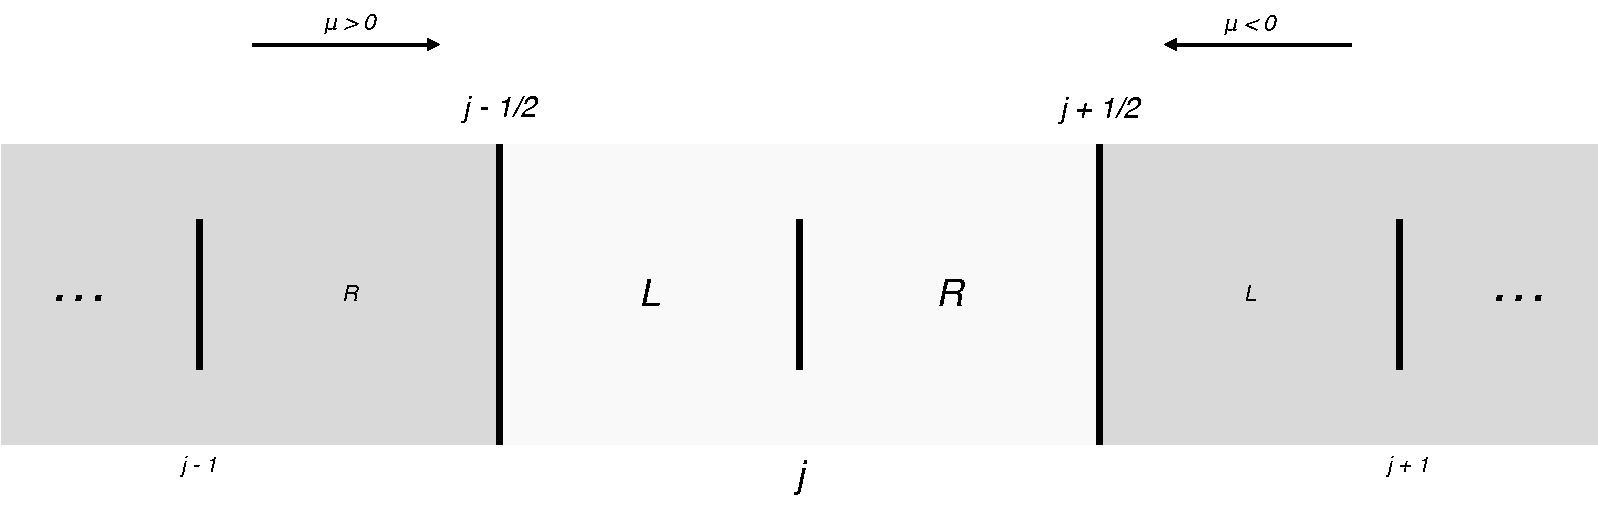
\includegraphics[width=\linewidth]{figures/smm_paper/diag.pdf}
    \caption{discretization scheme indices; simple corner balance in slab geometry.}
    \label{fig:disc}
\end{figure}

Simple corner balance in 1D is a finite element method, so the standard Larsen four-step procedure may produce an inconsistent system of equations which can be algebraically complex to solve \cite{adams_fast_2002}.
In this work we use the modified Adams--Martin four-step procedure \cite{adams_1992_dsadfe} to derive a set of second-moment equations.
The modified four step procedure starts by:

{First:} take the 0$^{th}$ angular moments of equations \eqref{eq:scb}:
\begin{subequations}
\label{eq:zeroth}
\begin{equation}
\label{eq:zeroth_left}
    \left[ \frac{J_{j,L} + J_{j.R}}{2} - J_{j-1/2} \right] + \Sigma_{a,j} \frac{\Delta x_j}{2} \phi_{j,L} = \frac{\Delta x_j}{2} \frac{Q_{j,L}}{2} \; ,
\end{equation}
\begin{equation}
     \left[ J_{j+1/2} - \frac{J_{j,L} + J_{j,R}}{2} \right] + \Sigma_{a,j} \frac{\Delta x_j}{2} \phi_{j,R} = \frac{\Delta x_j}{2} \frac{Q_{j,R}}{2} \; ,
\end{equation}
\end{subequations}
where $J$ is the total current (first angular moment). The upstream closure on the right cell edge is
\begin{subequations}
\label{edgescalar}
\begin{equation}
   \phi_{j+1/2} = \sum\limits_{\mu_{m}>0} w_m   \psi_{m,j,R}+\sum\limits_{\mu_{m}<0} w_m \psi_{m,j+1,L} \;,
\end{equation}
and the left is
\begin{equation}
   \phi_{j-1/2} = \sum\limits_{\mu_{m}>0} w_m   \psi_{m,j-1,R}+\sum\limits_{\mu_{m}<0} w_m \psi_{m,j,L} \;.
\end{equation}
\end{subequations}

{Second}: take the 1$^{st}$ angular moments of equations \eqref{eq:zeroth}:
\begin{subequations}
\label{eq:first}
\begin{equation}
    \frac{1}{3} \left[ \frac{\phi_{j,L} + \phi_{j.R}}{2} - \phi_{j-1/2} \right] + \frac{2}{3} \left[ \frac{\Gamma_{j,L} + \Gamma_{j.R}}{2} - \Gamma_{j-1/2} \right] + \Sigma_{t,j} \frac{\Delta x_j}{2} J_{j,L} = 0 \;
\end{equation}
\begin{equation}
    \frac{1}{3} \left[ \phi_{j+1/2} - \frac{\phi_{j,L} + \phi_{j,R}}{2} \right] +\frac{2}{3} \left[ \Gamma_{j+1/2} - \frac{\Gamma_{j,L} + \Gamma_{j,R}}{2} \right] + \Sigma_{t,j} \frac{\Delta x_j}{2} J_{j,R} = 0 \; ,
\end{equation}
where
\begin{equation}
    \Gamma =  \sum\limits_{m=1}^N w_m   P_2(\mu_m) \psi_{m} = \sum\limits_{m=1}^N w_m \left[ \frac{1}{2} \left( 3 \mu_m^2 - 1 \right) \right]  \psi_{m} \; 
\end{equation}
\end{subequations}
is the second angular moment.
The upstream closure on the right cell edge becomes
\begin{subequations}
\label{eq:edgecurrent}
\begin{equation}
   J_{j+1/2} = \sum\limits_{\mu_{m}>0} \mu_m w_m   \psi_{m,j,R}+\sum\limits_{\mu_{m}<0} \mu_m w_m \psi_{m,j+1,L}  \; ,
\end{equation}
and the left cell edge
\begin{equation}
   J_{j-1/2} = \sum\limits_{\mu_{m}>0} \mu_m w_m   \psi_{m,j-1,R}+\sum\limits_{\mu_{m}<0} \mu_m w_m \psi_{m,j,L}  \; .
\end{equation}
\end{subequations}

{Third:}, we {modify} Eq. (\ref{edgescalar}) to yield a local expression for the current, one that involves only the scalar fluxes in the cell
\begin{subequations}
\label{eq:modification}
\begin{equation}
    \phi_{j-1/2} = \phi_{j,L} \; ,
\end{equation}
and 
\begin{equation}
    \phi_{j+1/2} = \phi_{j,R} \; ,
\end{equation}
\end{subequations}
then insert into equations into Eqs. \eqref{eq:first}:
\begin{subequations}
\label{eq:current}
\begin{equation}
    J_{j,L} = - \frac{1}{3 \Sigma_{t,j} \Delta x_j} \left[ \phi_{j,R} - \phi_{j,L} \right] - \frac{4}{3 \Sigma_{t,j} \Delta x_j} \left[ \frac{\Gamma_{j,L} + \Gamma_{j,R}}{2} - \Gamma_{j-1/2} \right] 
\end{equation}
\begin{equation}
    J_{j,R} = - \frac{1}{3 \Sigma_{t,j} \Delta x_j} \left[ \phi_{j,R} - \phi_{j,L} \right] -\frac{4}{3 \Sigma_{t,j} \Delta x_j} \left[ \Gamma_{j+1/2} - \frac{\Gamma_{j,L} + \Gamma_{j,R}}{2} \right].
\end{equation}
\end{subequations}
We expand the cell edge currents from Eqs. \ref{eq:edgecurrent} using the P$_1$ approzetamation
\begin{subequations}
\begin{equation}
    J_{j+1/2} = \sum\limits_{\mu_{m}>0} \mu_m w_m   \left(\frac{1}{2} \phi_{j,R} + \frac{3\mu_m}{2} J_{j,R} \right)+\sum\limits_{\mu_{m}<0} \mu_m w_m \left(\frac{1}{2} \phi_{j+1,L} + \frac{3\mu_m}{2} J_{j+1,L} \right)
\end{equation}
and
\begin{equation}
    J_{j-1/2} = \sum\limits_{\mu_{m}>0} \mu_m w_m   \left(\frac{1}{2} \phi_{j-1,R} + \frac{3\mu_m}{2} J_{j-1,R} \right)+\sum\limits_{\mu_{m}<0} \mu_m w_m \left(\frac{1}{2} \phi_{j,L} + \frac{3\mu_m}{2} J_{j,L} \right)
\end{equation}
\end{subequations}
which simplify to
\begin{subequations}
\label{eq:edgecur}
\begin{equation}
    J_{j+1/2} = \gamma \left( \phi_{j,R} - \phi_{j+1,L} \right) + \zeta \left( J_{j,R} + J_{j+1,L} \right) \; ,
\end{equation}
and
\begin{equation}
    J_{j-1/2} = \gamma \left( \phi_{j,R-1} - \phi_{j,L} \right) + \zeta \left( J_{j-1,R} + J_{j,L} \right) \; ,
\end{equation}
where
\begin{equation}
    \gamma = \frac{1}{2} \sum\limits_{\mu_{m}>0} \mu_m w_m \approx \frac{1}{4} \; ,
\end{equation}
and
\begin{equation}
    \zeta = \frac{3}{2} \sum\limits_{\mu_{m}>0} \mu_m^2 w_m \approx \frac{1}{2} \; .
\end{equation}
\end{subequations}
For both constants $\zeta$ and $\gamma$ this is true in the limit of the number of quadrature points taken to infinity.

{Fourth:} combine Eqs. \eqref{eq:zeroth}, \eqref{eq:current} and \eqref{eq:edgecur} to form a system of equations
\begin{subequations}
\label{eq:full_secondmomemnt}
\begin{multline}
    -\left(1-\zeta \right) D_j \frac{\left( \phi_{j,R} - \phi_{j,L} \right)}{\zeta x_j} -\gamma \left( \phi_{j-1,R} - \phi_{j,L} \right) + \zeta D_{j-1} \frac{\left( \phi_{j-1,R} - \phi_{j-1,L} \right)}{\Delta x_{j-1}}
    \\
    + \Sigma_{a,j} \frac{\Delta x_j}{2} \phi_{j,L} = \frac{\Delta x_j}{2} \frac{Q_{j,L}}{2} +\frac{2 \zeta D_j}{\Delta x_j} \left(\Gamma_{j+1/2} - \Gamma_{j-1/2} \right)
    \\
     - \zeta \left[ \frac{4 D_j}{\Delta x_j} \left( \frac{\Gamma_{j,L} + \Gamma_{j,R}}{2} - \Gamma_{j-1/2} \right) + \frac{4 D_{j-1}}{\Delta x_{j-1}} \left(\Gamma_{j-1/2} -  \frac{\Gamma_{j-1,L} + \Gamma_{j-1,R}}{2} \right) \right] \; ,
\end{multline}
and
\begin{multline}
    \left(1-\zeta \right) D_j \frac{\left( \phi_{j,R} - \phi_{j,L} \right)}{\Delta x_j} +\gamma \left( \phi_{j,R} - \phi_{j+1,L} \right) - \zeta D_{j+1} \frac{\left( \phi_{j+1,R} - \phi_{j+1,L} \right)}{\Delta x_{j+1}}
    \\
    + \Sigma_{a,j} \frac{\Delta x_j}{2} \phi_{j,R} = \frac{\Delta x_j}{2} \frac{Q_{j,R}}{2} -\frac{2 \zeta D_j}{\Delta x_j} \left(\Gamma_{j+1/2} - \Gamma_{j-1/2} \right)
    \\
    + \zeta \left[ \frac{4 D_j}{\Delta x_j} \left( \Gamma_{j+1/2} - \frac{\Gamma_{j,L} + \Gamma_{j,R}}{2}  \right) + \frac{4 D_{j+1}}{\Delta x_{j+1}} \left( \frac{\Gamma_{j+1,L} + \Gamma_{j+1,R}}{2} - \Gamma_{j+1/2} \right)  \right] \;.
\end{multline}
\end{subequations}

A standard DSA method will discard the second moments and define the source ($Q$) as the error between subsequent iteration (commonly denoted by $\Delta \phi=\phi\la-\phi\lph$).
So the diffusion equations solve for an error estimation scalar flux which can be added to $l+1/2$ quantities to correct them.
In this analysis we use the Yavuz--Larsen method \cite{yavuz_spatial_1989} and keep the second moments as we solve for physical terms to update $l+1/2$ quantities, \textit{not} an error corrections.
Furthermore we can make a simplification that the second moments incident on the boundary of each cell are
\begin{subequations}
\label{eq:simple}
\begin{equation}
    \Gamma_{j-1/2} = \Gamma_{j,L}\lph \; 
\end{equation}
and
\begin{equation}
    \Gamma_{j+1/2} = \Gamma_{j,R}\lph \; ,
\end{equation}
\end{subequations}
so only within cell information is used.
This is similar to the modification the Adams--Martin method makes for the zeroth angular moment in Eqs. \eqref{eq:modification}.
% This simplifies the equations for the within cell currents:
% \begin{equation}
%     J_{j,L} = J_{j,R} = - \frac{1}{3 \Sigma_{t,j} \Delta x_j} \left[ \phi_{j,R} - \phi_{j,L} \right] - \frac{4}{3 \Sigma_{t,j} \Delta x_j} \left[ \Gamma_{j,R} - \Gamma_{j,L}  \right],
% %    \label{fm1}
% \end{equation}
This simplifies Eqs. \eqref{eq:full_secondmomemnt} to be a left side
\begin{subequations}
\label{eq:simple_smom}
\begin{multline}
-\left(1-\zeta \right) D_j \frac{\left( \phi_{j,R}^{(l+1)} - \phi_{j,L}^{(l+1)} \right)}{\Delta x_j} -\gamma \left( \phi_{j-1,R}^{(l+1)} - \phi_{j,L}^{(l+1)} \right) + 
\\ 
\zeta D_{j-1} \frac{\left( \phi_{j-1,R}^{(l+1)} - \phi_{j-1,L}^{(l+1)} \right)}{\Delta x_{j-1}} 
+ \Sigma_{a,j} \frac{\Delta x_j}{2} \phi_{j,L}^{(l+1)} = \frac{\Delta x_j}{2} \frac{Q_{j,L}}{2} 
\\
+\frac{2D_j( 1- \zeta) }{\Delta x_j} \left(\Gamma_{j,R}^{(l+1/2)} - \Gamma_{j,L}^{(l+1/2)} \right) 
- \frac{2 \zeta D_{j-1}}{\Delta x_{j-1}} \left( \Gamma_{j-1,R}^{(l+1/2)} - \Gamma_{j-1,L}^{(l+1/2)} \right) \; ,
\end{multline}
and right side
\begin{multline}
\left(1-\zeta \right) D_j \frac{\left( \phi_{j,R}^{(l+1)} - \phi_{j,L}^{(l+1)}  \right)}{\Delta x_j} +\gamma \left( \phi_{j,R}^{(l+1)}  - \phi_{j+1,L}^{(l+1)}  \right) - \zeta D_{j+1} \frac{\left( \phi_{j+1,R}^{(l+1)}  - \phi_{j+1,L}^{(l+1)}  \right)}{\Delta x_{j+1}} \\
+ \Sigma_{a,j} \frac{\Delta x_j}{2} \phi_{j,R}^{(l+1)}  = \frac{\Delta x_j}{2} \frac{Q_{j,R}}{2} \\
-\frac{2 D_j(\zeta-1)}{\Delta x_j} \left(\Gamma_{j,R}^{(l+1/2)} - \Gamma_{j,L}^{(l+1/2)} \right) + \frac{2 \zeta D_{j+1}}{\Delta x_{j+1}} \left(\Gamma_{j+1,R}^{(l+1/2)} - \Gamma_{j+1,L}^{(l+1/2)}\right)  \; ,
\end{multline}
\end{subequations}
balance which are written for a mid-step update to scalar flux and use only information coming from within a cell from the high-order transport solution.
Substituting Eq. \eqref{eq:simple} into Eq. \eqref{eq:current} forms the updated half-cell volume integrated currents 
\begin{equation}
\label{eq:simp_current}
    J_{j,L}^{(l+1)} = J_{j,R}^{(l+1)} = - \frac{1}{3 \Sigma_{t,j} \Delta x_j} \left[ \phi_{j,R}^{(l+1)} - \phi_{j,L}^{(l+1)} \right] - \frac{4}{3 \Sigma_{t,j} \Delta x_j} \left[ \Gamma_{j,R}^{(l+1/2)} - \Gamma_{j,L}^{(l+1/2)}  \right] \;.
%    \label{fm1}
\end{equation}


\subsection{Boundary Conditions}

We first develop boundary conditions for an incident angular flux on a given surface, then describe conditions on a reflecting surface.
Eq. \eqref{eq:zeroth_left} in the first cell ($j=1$) is
\begin{equation}
 \left[ \frac{J_{1,L} + J_{1,R}}{2} - J_{1/2} \right] + \Sigma_{a,1} \frac{\Delta x_1}{2} \phi_{1,L} = \frac{\Delta x_1}{2} \frac{Q_{1,L}}{2}. 
\end{equation}
On the left edge, the current ($J_{1/2}$) is a combination of the incident partial current, which is computed from the known incoming angular flux, and the outgoing partial current, which is computed using the P$_1$ expansion of the angular flux $\psi_{m,1,L}$:
\begin{equation}
    J_{1/2}= J^{-}_{\text{left}} - \left(\gamma \phi_{1,L} - \zeta J_{1,L}\right) \; ,
\end{equation}
where $J^{-}_{\text{left}}$ is the physical boundary condition imposed at the left boundary $j=1/2$.
Using the definition of $J_{1,L}$ from Eq. \eqref{eq:simp_current}, we find the first equation in the second-moment system is
\begin{subequations}
\label{eq:bc_inc}
\begin{multline}
    -\left(1-\zeta \right) D_1 \frac{\left( \phi_{1,R} - \phi_{1,L} \right)}{\Delta x_1} +\gamma  \phi_{1,L}  + \Sigma_{a,1} \frac{\Delta x_1}{2} \phi_{1,L} 
    \\ = 
    \frac{\Delta x_1}{2} \frac{Q_{1,L}}{2} +J^{-}_{\text{left}}+ 
    \frac{2D}{\Delta x}(\Gamma_{1,R}-\Gamma_{1,L}) \; .
\end{multline}
Likewise an incident angular flux boundary condition on the for the right ($j=I$) is
\begin{multline}
    \left(1-\zeta \right) D_I \frac{\left( \phi_{I,R} - \phi_{I,L} \right)}{\Delta x_I} +\gamma \left( \phi_{I,R}   \right)
    + \Sigma_{a,I} \frac{\Delta x_I}{2} \phi_{I,R}\\ = 
    \frac{\Delta x_I}{2}\frac{Q_I}{2} + J_{\text{right}}^+ - \frac{2 D_I}{\Delta x} \left( \Gamma_{I,R} - \Gamma_{I,L}\right) \; ,
\end{multline}
\end{subequations}
and is the final equation in the second-moment system.

Similarly we can define reflecting (Neumann) boundary conditions at $x=0$, $J_{1/2} = 0$, and this naturally is incorporated into the balance equation for the left-half of cell $j=1$.
Equation \eqref{eq:zeroth_left} in the first cell ($j=1$) then becomes
\begin{equation}
 \left[ \frac{J_{1,L} + J_{1,R}}{2} \right] + \sigma_{a,1} \frac{\Delta x_1}{2} \phi_{1,L} = \frac{\Delta x_1}{2} \frac{Q_{1,L}}{2}. 
\end{equation}
Inserting the definitions of $J_{1,L}$ and $J_{1,R}$ from Eq. \eqref{eq:simp_current} yields
\begin{subequations}
\begin{equation}
    - D_1 \frac{\left( \phi_{1,R} - \phi_{1,L} \right)}{\Delta x_1}  + \Sigma_{a,1} \frac{\Delta x_1}{2} \phi_{1,L} = \frac{\Delta x_1}{2} \frac{Q_{1,L}}{2} + 
    \frac{2D_1}{\Delta x}(\Gamma_{1,R}-\Gamma_{1,L}) \; .
\end{equation}
With reflecting boundary conditions the right hand side of cell $(j=I)$ is
\begin{equation}
    D_I \frac{\left( \phi_{I,R} - \phi_{I,L} \right)}{\Delta x_I}  + \Sigma_{a,I} \frac{\Delta x_I}{2} \phi_{I,R} = \frac{\Delta x_I}{2} \frac{Q_{I,R}}{2} + 
    \frac{2D_I}{\Delta x}(\Gamma_{I,R}-\Gamma_{I,L}) \; .
\end{equation}
\end{subequations}

\subsection{Cell-wise updates}

The preceding sections have described a system updating scalar flux and current.
Unlike SI which iterates on the scalar flux, OCI iterates exclusively on the angular flux.
Implementations of OCI algorithms may never form the scalar flux while iterating.
This is one of the challenges to finding a low-order transport approzetamation to aid in converging a higher-order OCI solve.
Normal acceleration methods only provide updates for \textit{moments} of angular flux in the sourcing side of the equation for the next iteration.

We use the update from the Yavuz-Larsen domain decomposition method to update all incident angular fluxes on the surfaces of all cells by
\begin{equation}
    \label{eq:update}
    \af\lp_{m,j,L/R} = \af_{m,j,L/R}\lph + \frac{1}{2}\left[\left(\phi_{j,R/L}\lp - \phi_{j,R/L}\lph\right) + 3\mu_m\left(J_{j,L/R}\lp - J_{j,L/R}\lph\right)\right] \;.
\end{equation}
This update removes the zeroth- and first-order moments from the $l+1/2$ angular flux and replaces them with zeroth- and first-order moments from the solution of the second-moment equations to produce a new incident angular flux on all cell bounds for $l+1$.
Notably, the second-moment equations were driven by material properties and information from the high-order transport solution at $l+1/2$.
This solution is also commuted globally.

Once the update for all incident angular flux is found on all cells the algorithm can continue until
\begin{subequations}
\begin{equation}
\label{eq:convergence_crit}
    \left|\left|\psi^{(l+1)}-\psi^{(l)}\right|\right|_{2} < \epsilon(1-\rho_{e}) \; ,
\end{equation}
controlling for false convergence when spectral radius is near unity, where $\epsilon$ is the convergence tolerance and
\begin{equation}
\label{eq:spec_rad_est}
    \rho_{e} = \frac{\left|\left|{\psi}^{(l+1)}-{\psi}^{(l)}\right|\right|_{2}}{\left|\left|{\psi}^{(l)}-{\psi}^{(l-1)}\right|\right|_{2}} \; ,
\end{equation}
\end{subequations}
is an empirical estimation of the spectral radius computed at every iteration of a transport solve. 


\begin{algorithm}
\begin{algorithmic}[1]

    \State initial guess for $\psi$

    \While{not converged}

        \State $\psi\lph =$ OCI iteration using $\psi\la$

        \State compute half-cell volume $\phi\lph$, $J\lph$, and $\Gamma\lph$ from $\psi\lph$

        \State solve second-moment equations for $\phi\lp$ \Comment{Eq. \eqref{eq:simple_smom}}

        \State solve for updated currents $J\lp$ \Comment{Eq. \eqref{eq:simp_current}}

        \State compute new angular fluxes using the Yavuz--Larsen update \Comment{Eq. \eqref{eq:update}}

        \State $e\lph=|\psi\lph - \psi\la|_2$

        \State $\rho_e = e\lph / e\la$ \Comment{Eq. \eqref{eq:spec_rad_est}}

        \If{$e^{(l)} < \epsilon(1-\rho_e)$} \Comment{Eq. \eqref{eq:convergence_crit}}
            \State converged = true
        \Else 

            \State $e\la = e\lph$
    
            \State $\psi\la = \psi\lp$ 
        \EndIf
    \EndWhile
    
    \caption{A one cell inversion iteration with second-moment method updating incident angular fluxes on the surface of every cell. Constructed so only a transport solution is used to measure error and test convergence.}
    \label{alg:smmoci}
\end{algorithmic}
\end{algorithm}


Algorithm \ref{alg:smmoci} shows how this second-moment method would be implemented with an OCI solve.
The OCI iteration is parallel over all angle and the block tri-diagonal diffusion matrix may be solved using any number of libraries optimized for execution on both CPU and GPU (e.g., cu/rocSPARSE \cite{cusparse, rocsparse}, MAGMA \cite{magma}, or others \cite{liwen_2012_solveable, klein_2023_tridiag}).
It has previously been shown that OCI algorithms lend themselves to implementation with linear algebra libraries which in-turn enables performance portability and more rapid methods development \cite{morgan_2025_oci}.
This remains the same when using the second moment algorithm shown in \ref{alg:smmoci}.


\section{Verification}

To verify that this method provides expected solutions, we use many anaclitic and benchmark problems with reference solutions.
We start by verifying the diffusion equations (setting second moments to zero) and verify using the method of manufactured solutions.
We compare the solutions computed by OCI and the second-moment method to a source free homogeneous slab (referenced to an SI solver), a three-region purely absorbing slab (referenced to an anaclitic solution), and a multi-region highly scattering slab (referenced to a highly resolved Monte Carlo result). 

Before confirming the full preconditioning scheme described in Section \ref{sec:methods} we use the method of manufactured solutions to verify the low-order diffusion equations produce the expected result \cite{warsa_mms_2010, moosemms}.
The diffusion equations for SCB are Equations \eqref{eq:full_secondmomemnt} with the contribution of the second moments neglected (as would be the case for traditional DSA).
Figure \ref{fig:diffusion_mms} shows the solution to linear and quadratic manufactured solutions.
To solve for a \textit{manufactured} source ($Q^m$) a \textit{manufactured} solution ($\phi^m$) can be produced and supplied to the continuous, one-speed, steady state, neutron diffusion equation
\begin{equation}
    -\frac{1}{3\Sigma}\frac{d^2\phi^m(x)}{dx^2} - \Sigma_a\phi(x)  = Q^m(x) \;.
\end{equation}
We then use $Q^m$ to produce half-cell volume integrated material sources over the problem domain ($x=[0,4]$\unit{\centi\meter}) with $\Sigma =$ \SI{10.0}{\per\centi\meter}, $\Sigma_s =$ \SI{5.0}{\per\centi\meter}, and $\Delta x =$ \SI{0.1}{\per\centi\meter}).
Figure \ref{fig:diffusion_mms} shows the diffusion equation matches manufactured solutions.
This demonstrates that the low-order diffusion equations are robust to nonphysical negative values.

\begin{figure}
    \centering
    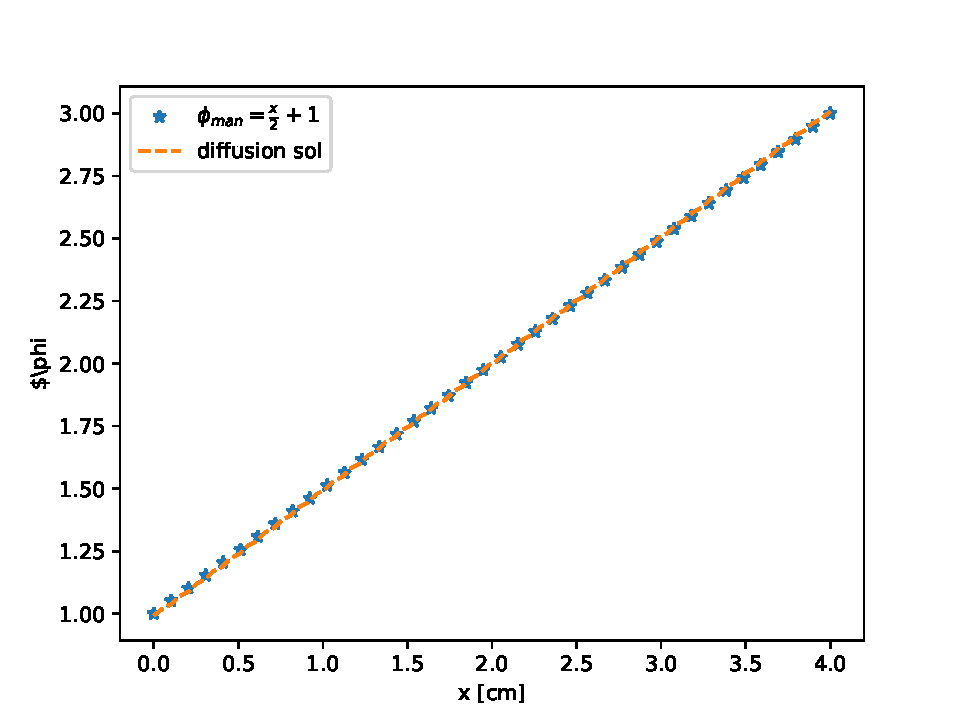
\includegraphics[width=.49\linewidth]{figures/smm_paper/linear_mms.pdf}
    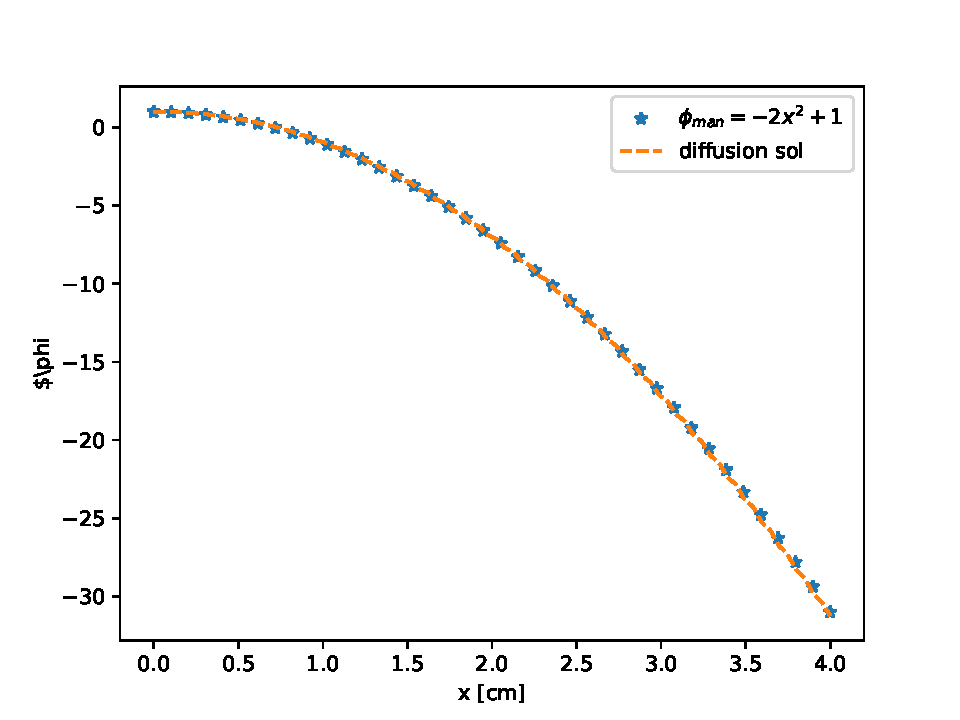
\includegraphics[width=.49\linewidth]{figures/smm_paper/quadratic_mms.pdf}
    \caption{Verification of the low-order diffusion equations using quadratic and linear manufactured solutions}
    \label{fig:diffusion_mms}
\end{figure}

To verify that our full second-moment equations produces the correct transport solutions we used a number of 1D benchmark problems.
We started with canonical transport problems including the infinite-homogeneous medium problem (using both reflecting and incident angular flux prescriptions) and the source-free pure absorber.
Both iterative methods converge to the expected analytical solutions for these problems.

Next, we consider three slab problems with increasing complezetaty.
First we use a \SI{4}{\centi\meter} wide source-free homogeneous slab where $\Sigma=$ \SI{1.0}{\per\centi\meter}, $\Sigma_s=$ \SI{0.5}{\per\centi\meter}, with an incident angular flux on the left of $\psi_{left}^-=$ \SI{5}{\per\centi\meter\cubed\per\s} and vacuum on the right.
In all work in this paper we use a convergence criterion of $\epsilon = $ \num{1e-5} and mazetamum iteration count of \num{2e4}.
We compare the solution from OCI and the second-moment method to one generated from a SI solver using a lumped-linear discontinuous finite element method.
In 1D, lumped-linear discontinuous is equivalent to the simple corner balance method we implement in this work \cite{adams_subcell_1997}.
Figure \ref{fig:regression_slab} compares the solution in both S$_2$ and S$_4$ showing a slight deviation between the two transport results and the second moment solution.
The number of iterations is shown in the legend of either plot.
In S$_2$ OCI takes 212 iterations whereas the second-moment method converges instantly (the solver forces at least 3 iterations).
We found that for all problems considered in S$_2$, the second-moment method will converge after a single iteration.
This is because the DSA equations are themselves the P$_1$ equations, which are equivariant to S$_2$ in 1D slab geometry.
In S$_4$ convergence is achieved after \num{197} and \num{127} iterations for OCI and the second-moment method, respectively.

\begin{figure}
    \centering
    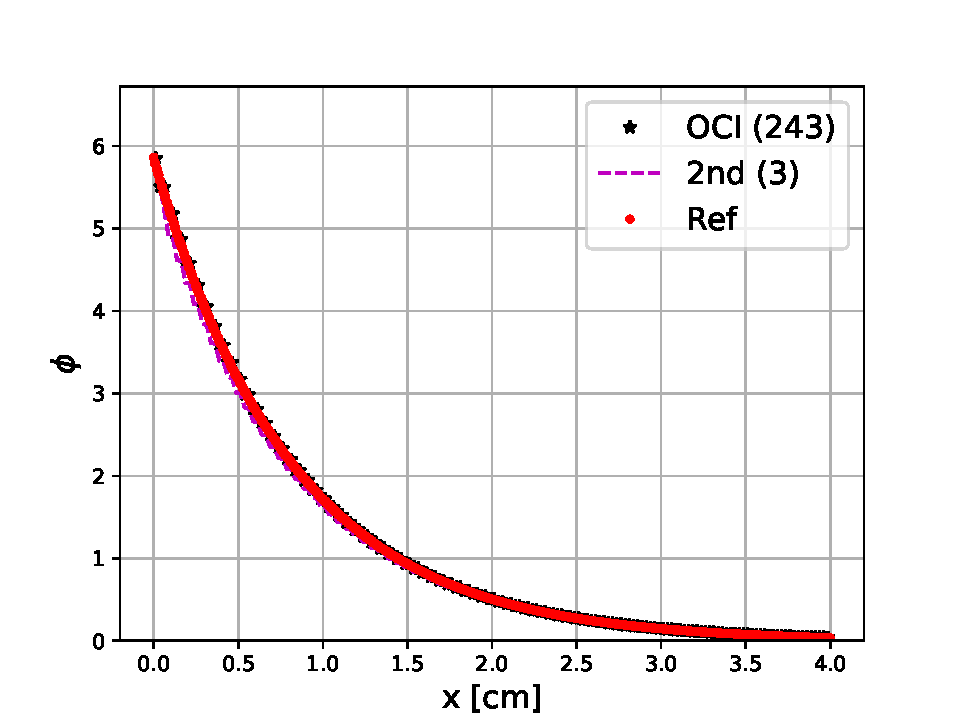
\includegraphics[width=.49\linewidth]{figures/smm_paper/regression_slabs2.pdf}
    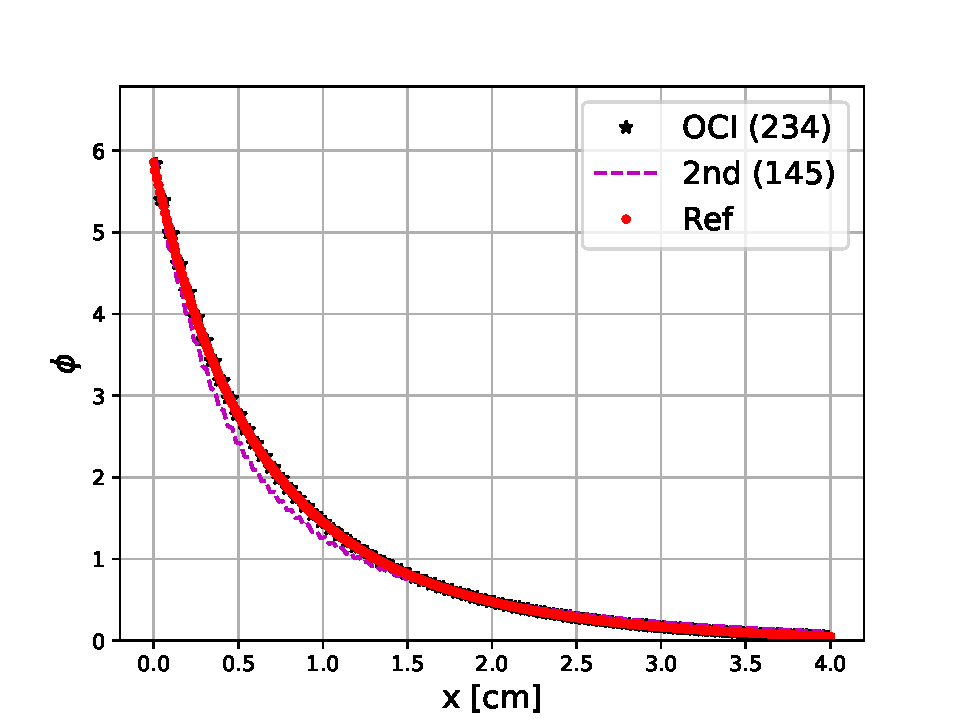
\includegraphics[width=.49\linewidth]{figures/smm_paper/regression_slabs4.pdf}
    \caption{Solution to a source free slab between OCI, the second-moment method, and a solution from a lumped linear discontinuous source iteration solver in S$_2$ (left) and S$_4$ (right).}
    \label{fig:regression_slab}
\end{figure}
 
Figure \ref{fig:absorbium} shows the solution for a three-region purely absorbing slab where $\Sigma = $ \qtylist{1.5; 2.0; 1.0}{\per\centi\meter} for region 1 ($\in$ \SI{0}{\centi\meter}--\SI{2}{\centi\meter}), 2 ($\in$ \SI{2}{\centi\meter}--\SI{4}{\centi\meter}) and 3 ($\in$ \SI{4}{\centi\meter}--\SI{6}{\centi\meter}), respectively.
An isotropic material source distributed throughout the whole problem domain ($Q=$ \SI{1.0}{\per\centi\meter\cubed\per\s}), with vacuum boundary conditions on the left and right, and we use $\Delta x =$ \SI{0.05}{\centi\meter} in S$_{16}$.
Figure \ref{fig:absorbium} at left shows $\phi$ for both OCI and the second-moment method as well as the solution from a closed forum anaclitic function.

The scalar fluxes match to within three decimal places, suggesting a matching solution.
However, Figure \ref{fig:absorbium} at right also shows angular flux as a function of both space and angle.
The transport solution seems to match the reference solution clearly; however, the second-moment method smears the solution appearing more rounded.
This may come from the assumed isotropy that is enforced at all cell incident cell interfaces. 
Notably this solution was archived in the same number of iterations for either method (\num{121}) suggesting the second-moment method provides no aid to $\rho$ without scattering.

\begin{figure}
    \centering
    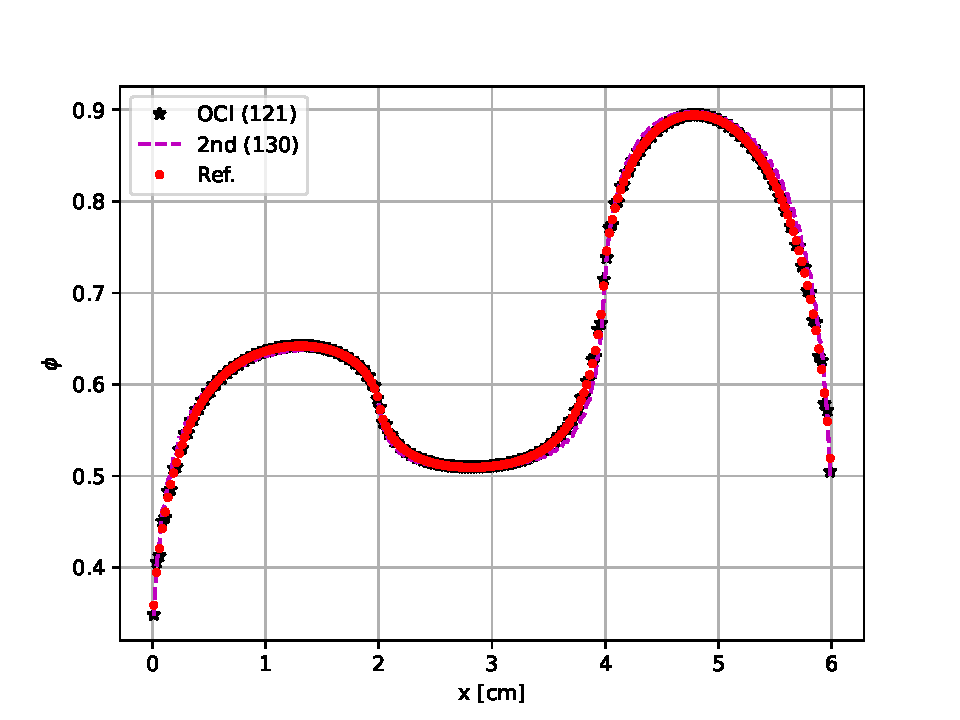
\includegraphics[width=.75\linewidth]{figures/smm_paper/slab_abs_sf.pdf}
    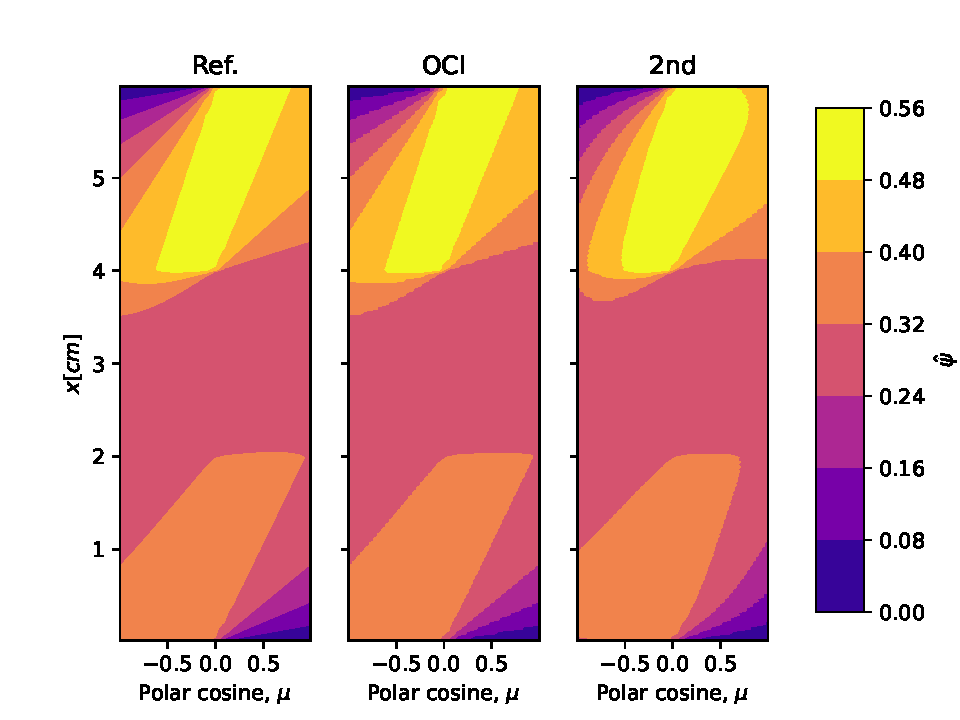
\includegraphics[width=.75\linewidth]{figures/smm_paper/slab_abs_af.pdf}
    \caption{Solution to the three-region purely absorbing slab problem with an anaclitic reference solution for $\phi$ (top) and $\psi$ (bottom) in S$_{16}$ with $\Delta x =$\SI{0.05}{\centi\meter}}
    \label{fig:absorbium}
\end{figure}

Finally, we consider a problem described by Yavuz and Larsen shown in Table \ref{tab:yavuz_problem} \cite{yavuz_spatial_1989}.
We solve this problem in the thin limit (using $\Delta x=$ \SI{0.01}{\centi\meter}) with a high quadrature order (S$_{32}$) and make comparisons to a Monte Carlo solution provided from MC/DC \cite{morgan_monte_2024}.
The Monte Carlo solution uses 100 evenly spaced tally bins in $x$ and 32 tally bins in polar angle, between $[-1, 1]$.
We ran this solution with \num{1e9} particles ran across 10 batches.
The L$_1$ norm of the variance computed over angles and space is \num{1.41e-3}.

\begin{table}
    \centering
    \begin{tabular}{cccc}
        \hline
        Region & Q \unit{\per\centi\meter\cubed\per\s} & $\Sigma$ \unit{\per\centi\meter} & $\Sigma_s$ \unit{\per\centi\meter}  \\
        \hline
        1 (\SI{0}{\centi\meter}--\SI{1}{\centi\meter}) & \num{0.0} & \num{1.0} & \num{1.00}\\
        2 (\SI{1}{\centi\meter}--\SI{2}{\centi\meter}) & \num{1.0} & \num{1.0} & \num{0.95}\\
        3 (\SI{2}{\centi\meter}--\SI{3}{\centi\meter}) & \num{1.0} & \num{1.0} & \num{0.80}\\
        4 (\SI{3}{\centi\meter}--\SI{4}{\centi\meter}) & \num{0.0} & \num{1.0} & \num{0.95}\\
        \hline
    \end{tabular}
    \caption{Yavuz and Larsen four-region highly scattering slab problem \cite{yavuz_spatial_1989}.}
    \label{tab:yavuz_problem}
\end{table}

Figure \ref{fig:yavuz} shows the results for ($\phi$ at left and $\psi$ at right) again between OCI, the second-moment method, and the reference Monte Carlo solution.
Note that all these solutions are normalized to compare to a Monte Carlo result which only provides shape solutions.
OCI matches the Monte Carlo solution.
The second-moment method again appears to deviate significantly starting in the lowest scattering region (region 3).
This is the spatially converged solution that does not noticeably change as $\Delta x \rightarrow 0$.
The angular flux appears smeared again suggesting an impact from low-order cell wise updates.
One thing to note is that OCI converges this problem in \num{3209} iterations where the second-moment method takes only \num{765}, a 4.2$\times$ reduction.

\begin{figure}
    \centering
    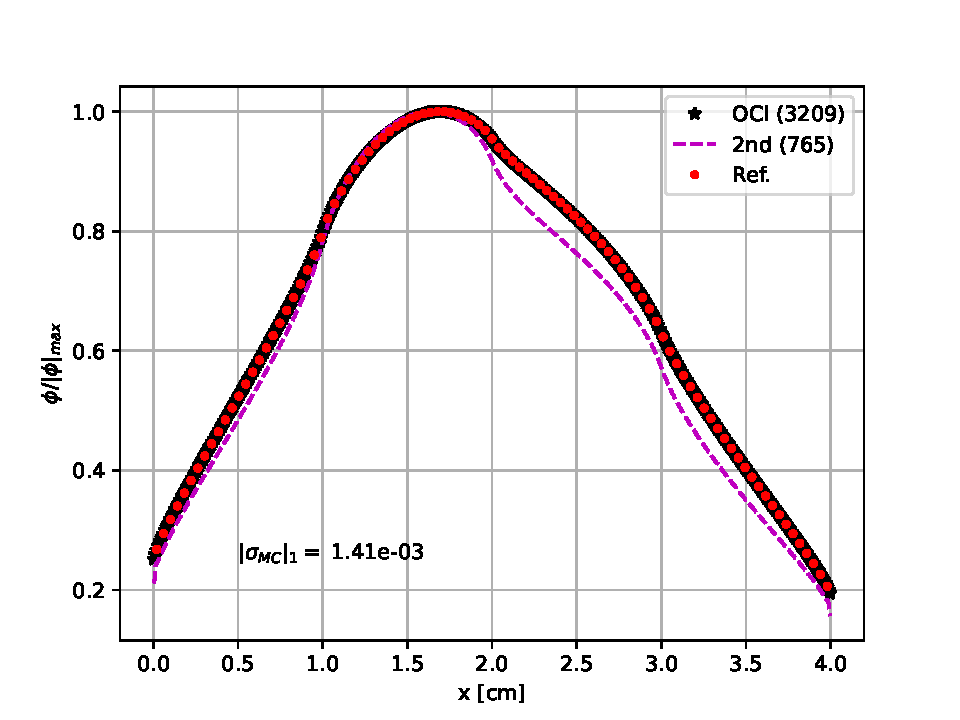
\includegraphics[width=.75\linewidth]{figures/smm_paper/yavuz_normalized_fluxes.pdf}
    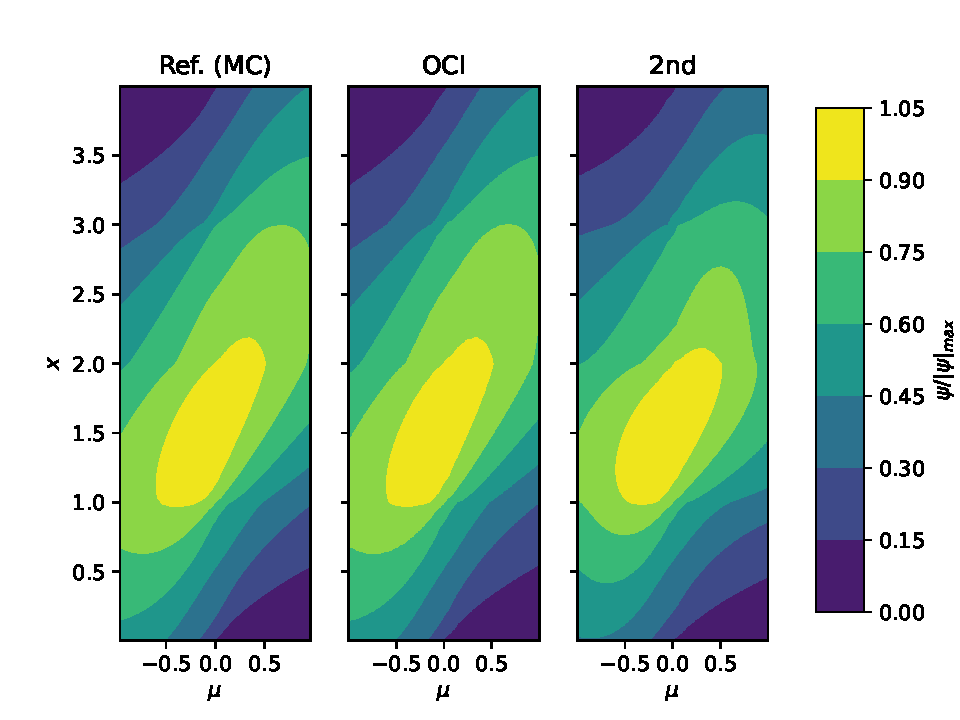
\includegraphics[width=.75\linewidth]{figures/smm_paper/yavuz_af.pdf}
    \caption{Normalized solutions to the Yavuz and Larsen problem via OCI, second-moment method, and Monte Carlo results for scalar flux (top) and angular flux (bottom) in S$_{32}$ with $\Delta x =$ \SI{0.01}{\centi\meter}. Solutions normalized to compare to Monte Carlo results.}
    \label{fig:yavuz}
\end{figure}

\section{Numerical Experiment}
\label{sec:num_exp}

To demonstrate the convergence behavior of the second-moment method across parameter space ($\delta \in [.01,10]$ and $c \in [0,1.0]$) we conduct a numerical experiment of a \SI{25}{\centi\meter} thick source-free infinite homogeneous slab with vacuum boundary conditions in S$_8$.
We hold all other parameters constant and vary $\delta$ and $c$ by varying $\Delta x$ and $\Sigma_s$ respectively.
For both algorithms we initialize the iteration randomly with $\psi^{0} \in [0, 1]$ to excite all error modes and measure error via the anaclitic (trivial solution)
\begin{equation}
    e^{(l)} = \left|\left|\psi^{(l)} - \bm{0}\right|\right|_2 \;.
\end{equation}
Spectral radius is then empirically measured with Equation \eqref{eq:spec_rad_est}.

\begin{figure}
    \centering
    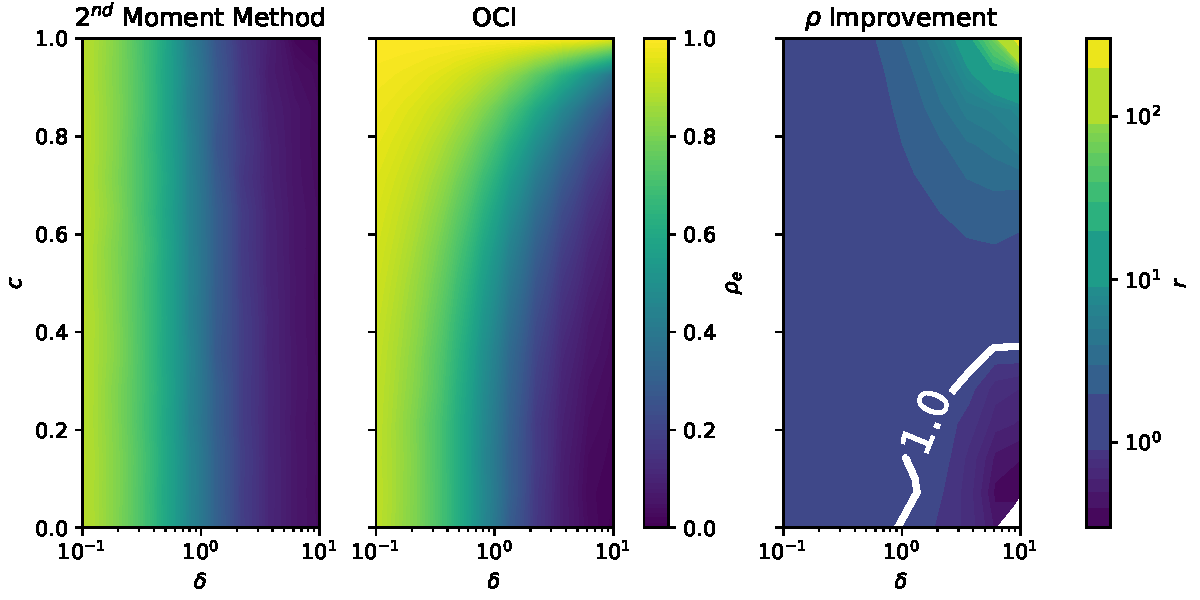
\includegraphics[width=\linewidth]{figures/smm_paper/smm_acc.pdf}
    \caption{Empirical estimations of spectral radius ($\rho_e$) over choices of parameter space for the second-moment method (left) and OCI (middle) from an infinite homogeneous medium problem in S$_8$ where $\psi^{0} \in [0,1]$. The ratio of $\rho_{OCI} / \rho_{SMM}$ (right), log color scale.}
    \label{fig:spec_rad}
\end{figure}

Figure \ref{fig:spec_rad} shows empirical measurements of spectral radius for the second-moment method (left) and OCI (middle) as functions of mean free path ($\delta$) and scattering ratio ($c$).
The measured spectral radius for OCI is the same as the solution provided via Fourier analysis in Figure \ref{fig:ss_spec_rads}.
The mazetamum spectral radius measured for OCI is \num{1.0} (OCI did not converge in the mazetamum iteration count) where the second moment is only \num{0.89}, potentially representing a difference of thousands of iterations. The second-moment method effectively eliminates convergence issues in the diffusive limit, making $\rho$ entirely a function of cellular optical thickness ($\delta$).
As expected it does not aid convergence in the thin limit. Figure \ref{fig:spec_rad} at right shows the ratio of
\begin{equation}
    \frac{\rho_{OCI}}{\rho_{SMM}} \; ,
\end{equation}
where $\rho_{OCI}$ and $\rho_{SMM}$ are the empirically measured spectral radii OCI and the second-moment method, respectively.
This clearly indicates the region where the second-moment method benefits convergence rate.
Everything to the left and above the line is where the ratio is $ > 1$, indicating the second-moment method is provides an improvement to spectral properties.
The most significant improvement is in the thick diffusive limit (upper right hand corner) which sees a mazetamum of 248$\times$ improvement in the parameter range we considered.
Marginal improvement is shown in most other regions---ratios between $1.0\times$ and $2.0\times$.
Decreased convergence rate is shown in the thick-streaming limit (lower right hand corner) where unpreconditioned OCI has exceptional convergence behavior.


\section{Discussion, Conclusions, and Future Work}

We use a second-moment domain decomposition method described by Yavuz and Larsen \cite{yavuz_spatial_1989} in conjunction with a one-cell inversion iteration \cite{rosa_cellwise_2013, morgan_2025_oci} in an effort to produce a fully space-parallel, rapidly convergent, transport iteration.
We derived and implemented the second-moment equations with OCI and a simple corner balance space discretization scheme.
A number of verification problems showed that the converged solution provided by the second-moment equations can deviate from transport and reference solutions.
We believe this is due to the simple within cell closures in Equations \label{eq:simple_close}.
When the full second-moment equations are implemented we do not expect the convergence behavior shown in Figure \ref{fig:spec_rad} to change significantly as it aligns with previous results when this method was used as a domain decomposition method for SI \cite{yavuz_spatial_1989}.

In S$_2$ the second moment scheme will converge after a single iteration.
This is because the DSA equations are themselves the P$_1$ expansions of the transport solution, in-turn equivalent to the S$_2$ equations in 1D.
The second-moment method seems to eliminate any dependence of the spectral radius ($\rho$) on scattering ratio ($c$) making it entirely a function of cellular optical thickness ($\delta$).
For optically thick this method is rapidly convergent regardless of scattering ratio.

For optically thin problems this second-moment method does not seem to aid convergence.
This agrees with previous work: Yavuz and Larsen state in their paper ``...although there is a degradation in the performance of the new SI and DSA [block Jacobi domain decomposition] algorithms as the size of the spatial subsystems decreases, this degradation is not serious until these subsystems are less than about a mean free path in diameter" \cite{yavuz_spatial_1989}. 
However, for optically thin time-dependent problems using OCI iterations we have already shown that small mean free times will push the spectral radius to zero \cite{morgan_2025_oci}.
So for highly time-dependent problems in the diffusive limit that demand significant temporal resolution, this second-moment-method may allow for rapidly convergent space-parallel transport iterations; however, this has yet to be shown.

We initially investigated a few synthetic acceleration schemes to converge OCI in both the scattering and thin-limits, including using a streaming-only problem as a low-order synthetic accelerator that can be computed parallel in space.
Fourier analysis for this acceleration method indicates that no acceleration would be provided by error corrections from the low-order problem.
TSA with $\beta=1$  uses a streaming+absorbing problem as a synthetic accelerator but requires a sweep \cite{tsa2009rosa}.
This leads us to suggest that the communication of quantities of interest interacting with cellular opacities is at minimum required for an acceleration scheme OCI in the thin limit.

Moving forward we will implement the full second-moment equations (without making within cell closures for second moments) in an attempt to rectify the inconsistencies.
We also plan to explore a standard DSA approach for solving mid-step updates of the zeroth and first angular moments, then assuming linear-anisotropy, use the update in Equation \ref{eq:update}.
We will also investigate the impact of GMRES to convergence rate.


\section*{Acknowledgments}

This work was supported by the Center for Exascale Monte-Carlo Neutron Transport (CEMeNT) a PSAAP-III project funded by the Department of Energy, grant number: DE-NA003967.